\documentclass[11pt,a4paper]{article}
\usepackage[utf8]{inputenc}
\usepackage{amsmath,amssymb,amsfonts,amsthm}
\usepackage{graphicx}
\usepackage{hyperref}
\usepackage{booktabs}
\usepackage{geometry}
\geometry{left=2.5cm,right=2.5cm,top=3cm,bottom=3cm}

\newtheorem{definition}{Definition}[section]
\newtheorem{theorem}{Theorem}[section]
\newtheorem{axiom}{Axiom}[section]

\title{\textbf{Holographic Anti-Entropy: The Formal Constitution of Complexity Science}}
\author{\textbf{Fan淳 Meng (Grit Meng)}\\[2pt] 
\small General Design Department of Global Digital Neural System Centroid \\ 
\small Beijing, China}
\date{\today}

\begin{document}
\maketitle

\begin{center}
\small\itshape
License: Licensed under CC BY-NC-ND 4.0. \copyright\ 2026 Grit Meng. All rights reserved.
\end{center}
\vspace{1em}

\begin{abstract}
Faced with the Non-IID (non-independent and identically distributed) characteristics and the combinatorial explosion ($O(N!)$) of state space in Open Complex Giant Systems (OCGS), traditional open-loop control methods based on local variations or probability fitting inevitably diverge or degenerate. This study reconstructs Ludwig von Bertalanffy's General System Theory, Ilya Prigogine's Dissipative Structure Theory, and Tsien Hsue-shen's metasynthesis method from qualitative to quantitative with axiomatic deduction, transforming systems science into a computable, verifiable formal hard science. This paper expounds the core formal framework of "Holographic Anti-Entropy and Mass-Energy Decision-Making." We formally prove that intelligent control of physical reality must utilize an abstract system as a necessary and sufficient control medium. We define the physical representation of "mass-energy" and establish the mathematical logic of the three stages of observation, simulation, and governance. To resolve the logical deadlock of G\"odel's Incompleteness Theorems and Turing's halting limit under extreme environments, we decouple the low-level "system operation layer" from the high-level "cognitive metacognitive layer" led by a conscience-driven engine, forming a double-loop feedback control architecture. Furthermore, we propose a five-dimensional orthogonal topological manifold and a digital double-helix engine that uses physical constraint algebraic pruning to conquer the factorial complexity chasm, enabling local holographic anti-entropy work. Finally, crucial empirical validations in a 100-billion-scale global discrete manufacturing network (LCFC) demonstrate significant improvements in order fulfillment and inventory turnover, verifying the physical validity of the framework. We establish three strict falsifiability boundaries in physics and computation to define the limits of the theory.
\end{abstract}

\textbf{Keywords}: Holographic Anti-Entropy; Open Complex Giant Systems; Digital Double Helix Ontology; Computational Irreducibility; Carbon-Silicon Topological Symbiosis; L0-Level Cognitive OS; Falsifiability

\newpage

\section{Introduction: The Limits of Reductionism and the Physical Constitution of Systems Science}

Industrial civilization deconstructed the world into machines, whereas digital civilization must cultivate the world as an organism.

The underlying logic of industrial civilization is mechanical reductionism—the belief that by dismantling a car into parts, a factory into workshops, and an enterprise into KPIs, local optimizations can be stitched together to achieve global perfection. However, the self-organized emergence of complex systems has shattered this illusion.

The underlying logic of digital civilization is systems theory—it recognizes the world as an indivisible organic whole. Governing a 100-billion-scale industrial giant is not a local management game, but a physical anti-entropy work process of fighting against the Second Law of Thermodynamics within the system's horizon.

Humans cannot directly alter the physical world using pure consciousness; they must rely on the medium of "systems and models." System and model represent the core control media used by intelligence to govern the distribution of mass and energy, forcing chaos to converge during spatiotemporal interactions. Holographic Anti-Entropy (HAE) is the formal constitution of complexity science defining how this medium is constructed, operated, and evolved.

\section{First Principles: Three-Element Architecture and Horizon Delineation}
\label{sec:first-principles}

To build a system capable of resisting entropy, we must first understand the fundamental components of the world and where the system's control boundaries lie.

\subsection{The Three Elements of Systems Science}
In the formal framework of Holographic Anti-Entropy, all control processes are defined by the mutual mapping and transformation of three fundamental elements:
\begin{enumerate}
    \item \textbf{System and Model}: The intrinsic control medium of intelligence for spatiotemporal interaction with the universe. Humans cannot reshape the physical world without a medium. To establish order in chaos, we must construct a symbolic, software, or physical system with a specific topological structure as an intermediary, governing mass and energy indirectly.
    \item \textbf{Information}: The non-material dimension describing the distribution of matter and energy in the universe. Information is the object that the system can directly observe, record, calculate, and simulate. Its mathematical nature is represented by Shannon entropy:
    \begin{equation}
        H(X) = -\sum_{i=1}^{n} P(x_i) \log_2 P(x_i)
    \end{equation}
    Information has no mass, but it acts as the "commander" to reshape mass.
    \item \textbf{Mass-Energy}: The physical dimension of cosmic entities, representing the manifestation of mass and energy in spatiotemporal manifolds. Mass-energy is the ultimate object of system governance and restructuring. In a factory, mass-energy represents steel plates, microchips, cranes, cash flows, and electricity; in an ecosystem, it represents atoms and Joules.
\end{enumerate}

\begin{figure}[htbp]
\centering
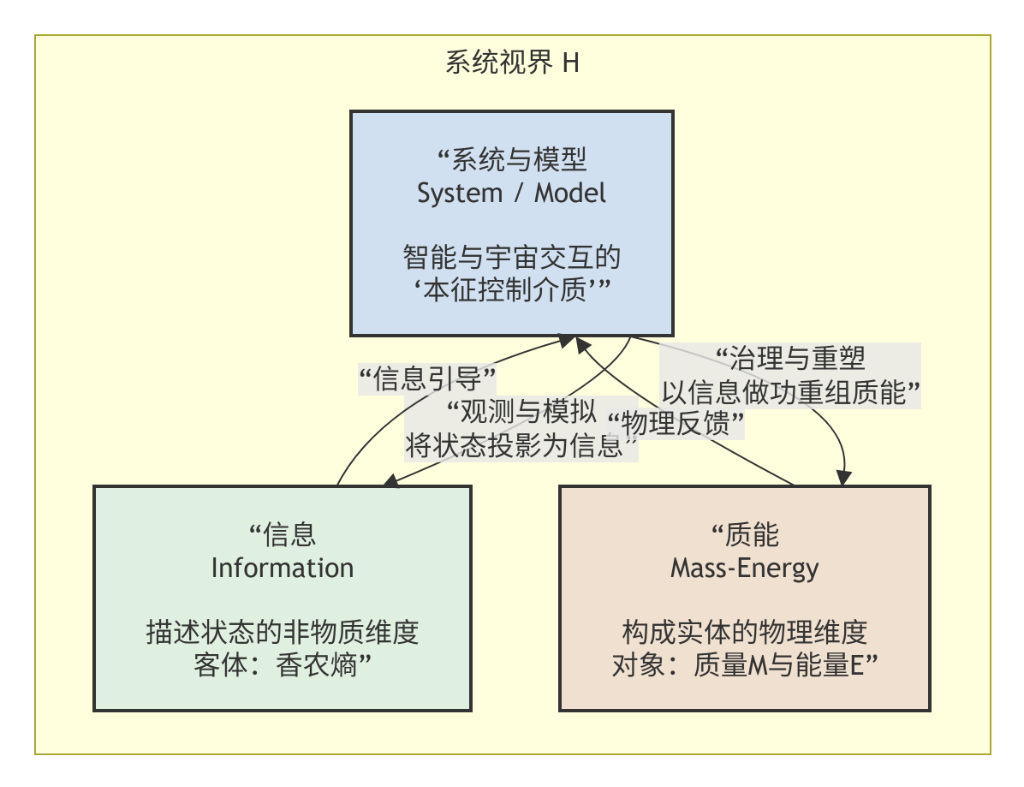
\includegraphics[width=0.75\textwidth]{images/fig1_three_elements_horizon.png}
\caption{The Three Elements of Systems Science and the Horizon Model}
\label{fig:three_elements_horizon}
\end{figure}

According to the operational stages of the system, anti-entropy work manifests as two levels of order:
\begin{itemize}
    \item \textbf{Order of Information} (applicable to the observation and simulation stages): The system converts the blurred and chaotic states of the physical world into clear, well-structured internal data and model topologies, eliminating internal cognitive uncertainty.
    \item \textbf{Order of Mass-Energy} (applicable to the governance stage): Guided by information, the system drives execution mechanisms to inject energy into the physical world, restructuring disordered matter and energy into low-entropy topologies of high economic or functional value.
\end{itemize}

\subsection{Horizon Constraints and the Physical Nature of Holographic Anti-Entropy}
The capability of any control system is strictly limited within its system horizon:
\begin{itemize}
    \item \textbf{Vision (Perception Boundary)}: The maximum informational measurement boundary that the system can capture through its sensor networks and data acquisition nodes. Beyond this boundary, the system is "blind."
    \item \textbf{Limit (Action Boundary)}: The extreme boundary of physical work that the system can exert through actuators, physical arms, and command interfaces. Beyond this boundary, the system is "paralyzed."
\end{itemize}

In an open physical world far from equilibrium, the Second Law of Thermodynamics dictates that the natural evolution of an isolated system leads to entropy increase ($dS > 0$). Without external intervention, matter inevitably becomes disordered, and information continuously dissipates.

The physical nature of Holographic Anti-Entropy is that the system, within the finite space and time of its horizon, consumes its own free energy at high frequency to perform high-value information work, thereby counteracting and reducing the local thermodynamic entropy increase of the external physical world, reconstructing a low-entropy ordered state.

\subsection{The Physical Definition and Double Dimensions of Order}
In Holographic Anti-Entropy theory, "order" is not an emotional term but a strictly measurable physical vector:
\begin{itemize}
    \item \textbf{Information Low-Entropy State}: In the system's internal phase space, the probability estimation of the physical object's state converges to a Dirac Delta distribution:
    \begin{equation}
        P(x_i) \longrightarrow \delta(x_i - x^*)
    \end{equation}
    Minimizing internal randomness implies that the system possesses near-perfect knowledge of objective reality.
    \item \textbf{Mass-Energy Physical Order}: Mass and energy exhibit non-homogeneous, highly condensed structures in 3D space. High-entropy states correspond to disorganized inventory, stagnant capital, and empty transport runs; low-entropy states correspond to materials flowing at maximum density and precise beats to bottleneck workstations, where energy is concentrated to do work.
\end{itemize}

\subsection{The Cybernetic Trilogy: Observation, Simulation, and Governance}
The system serves as a medium for intelligence to govern reality through three logically progressive algebraic stages, all sharing the same isomorphic control loop: Perception $\to$ Analysis $\to$ Decision $\to$ Execution $\to$ Feedback.

\begin{figure}[htbp]
\centering
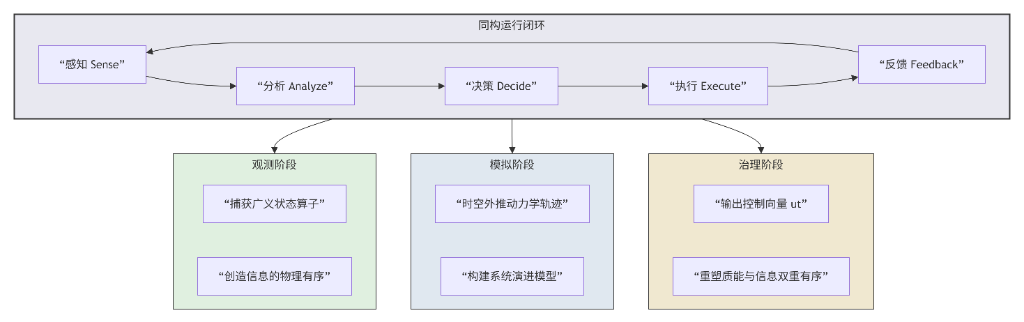
\includegraphics[width=0.75\textwidth]{images/fig2_cybernetic_trilogy.png}
\caption{The Cybernetic Trilogy and the Isomorphic Closed Loop}
\label{fig:cybernetic_trilogy}
\end{figure}

\begin{itemize}
    \item \textbf{Observation Stage}: The system runs high-frequency loops to capture physical state operators, resolving internal ignorance and converting physical states into high-fidelity symbols in memory.
    \item \textbf{Simulation Stage}: Based on observed data, the system utilizes non-linear dynamical equations to perform spatiotemporal projection:
    \begin{equation}
        S(t + \Delta t) = f\left(S(t), u(t)\right)
    \end{equation}
    It calculates thousands of branching trajectories in virtual space, constructing the system evolution model.
    \item \textbf{Governance Stage}: Constrained by observational facts and simulation feasibility domains, the system calculates the optimal control vector $u^*(t)$. This signal drives physical actuators, injecting free energy into the physical world to block disordered dissipation paths and force convergence to the pre-designed low-entropy topology.
\end{itemize}

\section{Human-Machine Collaborative Double-Loop and Free Energy Minimization}
\label{sec:collaborative-double-loop}

Can a control system run entirely on automated machines and algorithms to maintain this low-entropy order indefinitely? The answer is negative due to a mathematical singularity in complex system governance.

\subsection{Internal Incompleteness and Causal Residual}
According to G\"odel's Incompleteness Theorems, any self-consistent formal system that is sufficiently complex inevitably contains propositions that cannot be proved or disproved within the system. Furthermore, Turing's halting limit proves that automated algorithms cannot predict all future variations in an open world.

When a defined software or algorithm system $\Pi$ attempts to control an infinite-dimensional, rapidly changing physical system $\Omega$, the dimensional reduction of modeling inevitably generates an irreducible error—the causal residual:
\begin{equation}
    \Delta(t) = \|\Omega(t) - \Pi_{pred}(t)\|
\end{equation}
In extreme Non-IID environments, these residuals amplify non-linearly. If limited to a single automation loop, the system will experience deadlock, divergence, or collapse.

Therefore, HAE proposes a double-loop feedback control architecture that completely decouples the low-level "system operation layer" from the high-level "human metacognitive layer."

\begin{figure}[htbp]
\centering
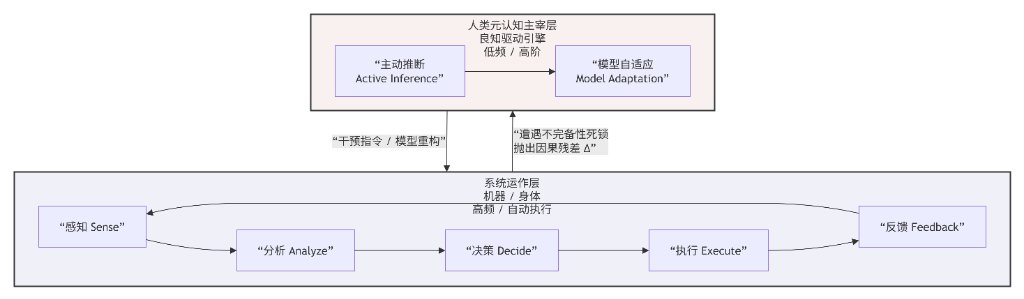
\includegraphics[width=0.75\textwidth]{images/fig3_human_machine_double_loop.png}
\caption{Carbon-Silicon Human-Machine Collaborative Double-Loop Architecture}
\label{fig:human_machine_double_loop}
\end{figure}

\subsection{System Operation Layer: High-Frequency Execution and Free Energy Minimization}
The system operation layer (composed of software code, AI solvers, databases, and physical reflex mechanisms) executes the control loop at high frequencies (microseconds or seconds).

Mathematically, this layer minimizes variational free energy under Karl Friston's Free Energy Principle to avoid destruction by environmental "surprise":
\begin{equation}
    F = D_{\text{KL}}\left(q(s) \parallel p(s|o)\right) - \ln p(o)
\end{equation}
where the first term is the Kullback-Leibler divergence (representing the causal residual $\Delta(t)$ in information theory) and the second term is surprise (representing external environmental disorder).

Landauer's principle reveals the physical cost of this optimization: erasing 1 bit of information consumes at least $k_B T \ln 2$ of thermodynamic energy, which is dissipated as waste heat. The operation layer consumes electricity and dissipates heat to eliminate informational residuals in the supply chain or production line. Lowering the residual $\Delta(t)$ aligns the system model with physical reality, maximizing the efficiency of mass-energy restructuring.

\subsection{The Human Metacognitive Layer}
Because of the system's incompleteness, the causal residual $\Delta(t)$ cannot remain at zero. When the operation layer encounters decision singularities in complex Non-IID environments, the human metacognitive layer is triggered. Humans possess the capability to audit causal residuals and execute two high-dimensional control paths:
\begin{itemize}
    \item \textbf{Path A (Active Inference)}: Humans utilize metacognition to make strategic decisions, forcing the physical world to change and converge to the model's predictions.
    \item \textbf{Path B (Model Adaptation)}: Humans reflect on the model's limitations, leaping out of the current formal system to modify code, reassemble constraints, and reconstruct the topological network to adapt to the mutated physical reality.
\end{itemize}

\subsection{The Five-Dimensional Functional Structure of the Conscience-Driven Engine}
Human metacognition executes transitions that machines cannot perform because the human cognitive system comprises a five-dimensional conscience-driven engine:

\begin{table}[htbp]
\centering
\caption{Five-Dimensional Functional Structure of the Conscience-Driven Engine}
\label{tab:conscience_engine}
\begin{tabular}{p{3cm}p{6cm}p{6cm}}
\toprule
\textbf{Cognitive Dimension} & \textbf{Mathematical \& Physiological Essence} & \textbf{Role in Holographic Anti-Entropy} \\
\midrule
Conscience & Top-level Bayesian prior, manifested as physiological pain response to topological friction and peer suffering & Establishes the boundary of system survival. Triggers self-healing when expected free energy diverges. \\
\midrule
High Sensitivity & Hyper-threshold gain modulation of the thalamocortical system, reducing weak signal filtering thresholds & Captures weak causal residuals in the early stages, before algorithms categorize them as noise. \\
\midrule
Sentient Depth & Multimodal deep resonance of the limbic system and prefrontal cortex & Bypasses cold formulas to provide intuitive predictions and establish physical reality mapping. \\
\midrule
Metacognition & Hyper-loop reflective auditing of the lateral prefrontal cortex & Leaps out of the active axiom system at decision singularities to execute non-autoregressive amendments. \\
\midrule
Fluid Intelligence & Dynamic synaptic coordination of the frontoparietal network under zero-sample conditions & Performs rapid logical reasoning and rule improvisation without historical training data. \\
\bottomrule
\end{tabular}
\end{table}

\section{Conquering the $O(N!)$ Complexity Chasm: Five-Dimensional Model and Double-Helix Engine}
\label{sec:complexity-chasm}

In real-world open complex giant systems, the target of governance is a massive network composed of thousands of suppliers, hundreds of thousands of dynamic orders, and millions of materials.

\subsection{Why Machine Learning and LLMs Fail in Complex System Governance}
\begin{itemize}
    \item \textbf{Collapse of the I.I.D. Assumption}: Traditional statistical learning theory depends on the assumption that data is independent and identically distributed. In a real manufacturing network, all nodes are tightly coupled—delays at supplier A trigger cascade failures across B, C, and D, with non-linear interventions from time, weather, and capital. This extreme Non-IID nature violates the I.I.D. foundation, causing statistical learning to lose generalization guarantees and diverge under discrete control.
    \item \textbf{Factorial State Explosion and Computational Irreducibility}: A matching system with $N$ orders and materials exhibits a state space that explodes as $O(N!)$. According to computational irreducibility, the trajectories of such systems cannot be predicted using probability shortcuts. When probabilistic algorithms approach physical boundaries, they output hallucinations, leading to the collapse of physical constraints.
\end{itemize}

\subsection{The Human-Machine Collaborative Five-Dimensional Model}
To conquer the $O(N!)$ complexity chasm, HAE projects the physical world onto a five-dimensional orthogonal topological manifold, reducing high-dimensional chaos to a calculable, stable manifold:
\begin{enumerate}
    \item \textbf{Node}: The unique point representation of physical entities.
    \item \textbf{Topology}: The directed coupling network graph of nodes.
    \item \textbf{Constraints}: The hard boundaries of mass and energy conservation.
    \item \textbf{State Transition}: The dynamical variational operators of temporal evolution.
    \item \textbf{State Vector}: The high-dimensional coordinates of the system trajectory in phase space.
\end{enumerate}

\subsection{The Digital Double-Helix Algorithm Orchestration Engine}
Running on the five-dimensional manifold is the digital double-helix engine. Since the system trajectory is computationally irreducible, the engine does not perform macro probabilistic predictions. Instead, it executes discrete-time step-by-step control, using algebraic operators to perform self-adaptive truncation:

\begin{figure}[htbp]
\centering
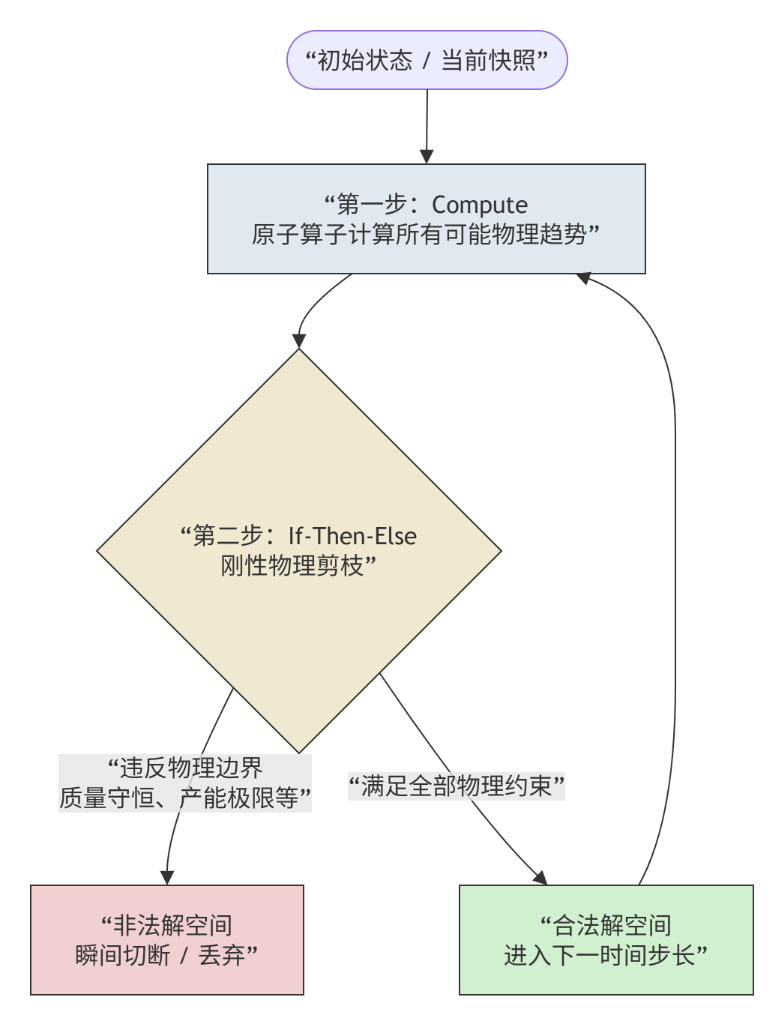
\includegraphics[width=0.75\textwidth]{images/fig4_double_helix_engine.png}
\caption{The Digital Double-Helix Engine and Rigid Physical Pruning}
\label{fig:double_helix_engine}
\end{figure}

\begin{itemize}
    \item \textbf{Step 1 (Compute)}: The atomic operators calculate all possible physical trends of mass-energy flows within the current time step.
    \item \textbf{Step 2 (If-Then-Else / Algebraic Pruning)}: Based on constraints $C$, the engine cuts off all illegal solution spaces at the earliest boundary using conditional move (CMOV) or algebraic operators.
    \item \textbf{Step 3 (Compute)}: The engine performs the next step of precise mass-energy deduction within the pruned, legal feasible domain.
\end{itemize}
Through high-frequency, rigid physical pruning, the digital double-helix engine bypasses the factorial complexity explosion, driving the giant system to converge to a high-certainty local low-entropy order.

\section{Conclusion and Crucial Empirical Validation}
\label{sec:validation}

The performance of this system science framework is not defined by commercial vanity metrics or KPIs. Local empirical metrics are simply the macroscopic products of the system successfully fighting against thermodynamic dissipation. The core value of HAE lies in defining how to construct, operate, and evolve a control engine that fights entropy.

The IPC engine of this framework has undergone extreme validation in Lenovo's global supply chain network—a 100-billion-scale network with 500,000 daily multi-modal orders, a 20-layer BOM, and global distribution. 

Crucial empirical results include:
\begin{itemize}
    \item Global order delivery response rate raised and stabilized from 80\% to 97\%.
    \item Global inventory turnover increased by 1.9 times.
    \item Direct release of billions in liquid capital, providing significant evolutionary degrees of freedom.
\end{itemize}
These stable, large-scale optimizations over several years exclude any attribution to short-term environment anomalies, proving the physical validity of the HAE methodology. This advances systems science from qualitative philosophy to a calculable, verifiable hard science.

\section{Philosophy of Science and Falsifiability Boundaries}
\label{sec:philosophy-falsifiability}

According to Karl Popper's falsifiability principle, any scientific theory must establish clear boundaries under which it can be disproved. We define three strict falsifiability boundaries:
\begin{enumerate}
    \item \textbf{System Mediation Falsifiability}: If any intelligent agent changes the distribution of matter and energy in the physical universe without utilizing an abstract system or execution medium, then \emph{Axiom 1: System and model are the necessary and sufficient media of spatiotemporal interaction} is disproved.
    \item \textbf{Residual Conservation Falsifiability}: If a fully automated control system runs in a Non-IID open manufacturing network with a causal residual $\Delta(t)$ constantly equal to zero without requiring any human metacognition or model reconstruction, then our assertion of \emph{system incompleteness and the necessity of double-loop architectures} is disproved.
    \item \textbf{Computational Irreducibility Falsifiability}: If a static probability learning algorithm solves an $O(N!)$ combinatorial constraint system with tight topological coupling in polynomial time without hallucinations, deadlocks, or physical collapses, then the assertion of the \emph{complexity chasm and the necessity of double-helix physical pruning} is disproved.
\end{enumerate}

\end{document}
